% statistics_and_probability:x17 GDC:YES
\begin{question}
  \hspace*{\fill} [Note maximale: 12]\par
  \medskip
  \noindent Deux dés équilibrés à quatre faces, l’un rouge et l’autre vert, sont jetés. Pour chaque dé, les faces sont marquées 1, 2, 3, 4. Le score pour chaque dé est le nombre sur la face sur laquelle le dé tombe.\par
  \medskip
  (a) Listez les paires de scores qui donnent une somme de 6.\hspace*{\fill} [3]\par
  \medskip
  \noindent La distribution de probabilités pour la somme des scores des deux dés est donnée ci-dessous.\par
  \medskip
  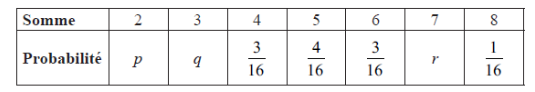
\includegraphics[scale=0.5]{tableau_sommes_des_scores}\par
  \medskip
  (b) Trouvez la valeur de p , de q et de r.\hspace*{\fill} [3]\par
  \medskip
  \noindent Fred joue à un jeu. Il lance quatre fois deux dés équilibrés à quatre faces. Il gagne un prix si la somme est 5 pour trois lancers ou plus.\par
  \medskip
  (c) Trouvez la probabilité que Fred gagne un prix.\hspace*{\fill} [6]\par
\end{question}

